\documentclass[a4paper,10pt]{article}

% ---------- Fonts and page layout ----------
% （注）フォント名は本環境（macOS + Tectonic）で解決できる表記に合わせ，
%  phase2 レポートの TeXGyreTermes / TeXGyreHeros をスペース入り正式名で指定している。
\usepackage{xeCJK}
\setmainfont{TeX Gyre Termes}
\setsansfont{TeX Gyre Heros}
\setmonofont{DejaVu Sans Mono}
\setCJKmainfont{Noto Serif CJK JP}
\setCJKsansfont{Noto Sans CJK JP}
\setCJKmonofont{Noto Sans Mono CJK JP}
\XeTeXlinebreaklocale "ja"
\XeTeXlinebreakskip=0pt plus 1pt

\usepackage[a4paper,left=24mm,right=24mm,top=24mm,bottom=25mm]{geometry}
\usepackage{setspace}
\setstretch{1.15}
\setlength{\parindent}{1em}
\setlength{\parskip}{0.25em}

% ---------- Math, tables, figures ----------
\usepackage{amsmath,amssymb,mathtools}
\usepackage{graphicx}
\usepackage{booktabs}
\usepackage{longtable}
\usepackage{tabularx}
\usepackage{array}
\usepackage{multirow}
\usepackage{makecell}
\usepackage{float}
\usepackage{caption}
\usepackage{xcolor}
\usepackage{enumitem}
\usepackage{titlesec}
\usepackage{fancyhdr}
\usepackage[hidelinks]{hyperref}
\usepackage{url}
\usepackage{microtype}
\usepackage[most]{tcolorbox}

\graphicspath{{figures/}}

% ---------- Unified style ----------
\definecolor{bbblack}{HTML}{222222}
\definecolor{bbgray}{HTML}{666666}
\definecolor{bblight}{HTML}{F2F2F2}
\definecolor{bbline}{HTML}{333333}
\renewcommand{\figurename}{Figure}
\renewcommand{\tablename}{Table}
\captionsetup{font={small},labelfont={bf},justification=raggedright,singlelinecheck=false}
\captionsetup[table]{position=top}
\captionsetup[figure]{position=bottom}
\renewcommand{\arraystretch}{1.22}
\setlist[itemize]{leftmargin=1.6em,itemsep=0.15em,topsep=0.2em}
\setlist[enumerate]{leftmargin=1.8em,itemsep=0.15em,topsep=0.2em}

\titleformat{\section}{\sffamily\bfseries\Large\color{bbblack}}{\thesection}{0.8em}{}
\titleformat{\subsection}{\sffamily\bfseries\large\color{bbblack}}{\thesubsection}{0.7em}{}
\titleformat{\subsubsection}{\sffamily\bfseries\normalsize\color{bbblack}}{\thesubsubsection}{0.6em}{}
\titlespacing*{\section}{0pt}{1.2em}{0.5em}
\titlespacing*{\subsection}{0pt}{0.9em}{0.35em}
\titlespacing*{\subsubsection}{0pt}{0.7em}{0.25em}

\pagestyle{fancy}
\fancyhf{}
\lhead{\small\sffamily BEYOND BUFFETT Phase4 Methodology}
\rhead{\small\sffamily 配分：役割予算×リスク調整}
\cfoot{\small\thepage}
\renewcommand{\headrulewidth}{0.4pt}

\newcolumntype{Y}{>{\raggedright\arraybackslash}X}
\newcommand{\metric}[1]{\mathrm{#1}}
\newcommand{\ind}[1]{\mathbf{1}\{#1\}}

\newtcolorbox{keybox}[1][]{
  colback=bblight, colframe=bblight, boxrule=0pt, arc=1mm,
  left=2mm, right=2mm, top=2mm, bottom=2mm, breakable,
  before skip=6pt, after skip=6pt,
  title={#1}, coltitle=bbblack, fonttitle=\sffamily\bfseries,
  attach title to upper={\par}
}
\newtcolorbox{defbox}[1][直感]{
  colback=white, colframe=bbline, boxrule=0.6pt, arc=1mm,
  left=2mm, right=2mm, top=2mm, bottom=2mm, breakable,
  before skip=6pt, after skip=6pt,
  title={#1}, coltitle=bbblack, fonttitle=\sffamily\bfseries,
  attach title to upper={\par}
}

\begin{document}

% ---------- Cover ----------
\begin{titlepage}
\centering
\vspace*{12mm}
{\sffamily\bfseries\Huge BEYOND BUFFETT\par}
\vspace{6mm}
{\sffamily\bfseries\LARGE Phase4 解説レポート\par}
\vspace{3mm}
{\sffamily\Large 配分：選定済み 20 社へ，成績予想を使わずに 500 万円を配る\par}
\vspace{14mm}
{\large 本資料は，Phase3 で確定した最終 20 社に対し，\par}
{\large 役割予算とリスク調整だけで目標比率を決め，\par}
{\large 単元株の丸めを経て実購入額に落とすまでを，0 から解説する。\par}
\vfill
{\small 正典データ：phase4\_portfolio\_allocation/allocation\_final.csv\par}
\end{titlepage}

\setcounter{tocdepth}{2}
\tableofcontents
\clearpage

% ---------- 1 ----------
\section{エグゼクティブサマリー}

Phase4 の目的は，どの銘柄を買うかではない。それは Phase3 で確定し，以後変更しない。ここで決めるのは「選定済みの 20 社へ，総予算 500 万円をどう配るか」だけである。

\begin{keybox}[Phase4 の一文定義]
\centering
\Large 選ばれた 20 社に，成績予想を使わず，説明できる形で 500 万円を配る。
\end{keybox}

配分は四段階で決めた。（i）20 社を役割ごとに分ける。（ii）役割ごとの予算を決める（完成・変化・新生の三世代に各 25\%，両立型 15\%，分散役 10\%）。（iii）同じ役割の中では，値動きが穏やかで・売買しやすく・証拠が強く・データが信頼できる会社を厚くする（式\eqref{eq:alloc}）。（iv）1 銘柄 8\% の上限と，実際に買える株数（式\eqref{eq:lot}）に丸める。結果は，投資額 4{,}949{,}198 円・残現金 50{,}801 円（予算消化率 99.0\%），最大保有はゼンリンの 7.46\% であった。リターンの予測は一切使っていない。

\section{この資料の読み方}

\ref{sec:whynot}節で「なぜ等金額で終わらせないのか」を確認し，\ref{sec:budget}節で役割予算，\ref{sec:tilt}節で役割内の傾け（式\eqref{eq:alloc}），\ref{sec:cap}節で 8\% 上限の配り直し，\ref{sec:lot}節で単元株の丸め（式\eqref{eq:lot}）を読む。\ref{sec:example}節の計算例で一社を 0 から追い，\ref{sec:limits}節の限界で締める。配分は「検証で良かったから増やす」という後知恵を含まない。

% ---------- 2 ----------
\section{なぜ等金額で終わらせないのか}
\label{sec:whynot}

最も単純な配分は等金額（各社 5\%）である。等金額は「どの会社も同じだけ信じる」という明確な思想であり，出発点として悪くない。しかし本研究の 20 社は，役割も，値動きの大きさも，売買のしやすさも，証拠の強さも異なる。これらを無視して同額を配ると，たとえば値動きの大きい銘柄がポートフォリオ全体の変動を支配してしまう。

検討した配分案は四つある。A 案：等金額。B 案：役割別予算（各役割内は均等）。C 案：役割別予算＋リスク調整（採用）。D 案：制約付き最小分散（参考）。

\begin{defbox}
役割構成が 5/5/5/3/2 のとき，B 案（役割予算 25/25/25/15/10 を役割内で均等割り）は各社 5\% となり，数学的に A 案と一致する。つまり等金額は「三世代を等しく信じる」という役割予算の特殊形として正当化できる。C 案はその一段階拡張である。
\end{defbox}

D 案（最小分散）は分散最小化としては優れるが，重みがブラックボックスになりやすく，特定業種へ 24\% まで集中する解が出たため，説明可能性を優先して参考にとどめた。

% ---------- 3 ----------
\section{役割予算：三世代へ等しく賭ける}
\label{sec:budget}

役割予算は，完成した堀・変わる堀・生まれる堀へ各 25\%，両立型 15\%，分散役 10\% とした。三世代へ同額を置くのは，どの未来（現在価値の実現・再評価・新市場の成長）が来ても土台が残るようにするためであり，リターン予想に基づく傾斜ではない。両立型は魅力的だが集中リスクがあるため 15\% に抑え，分散役は緩衝として 10\% とした。

\begin{figure}[H]
\centering
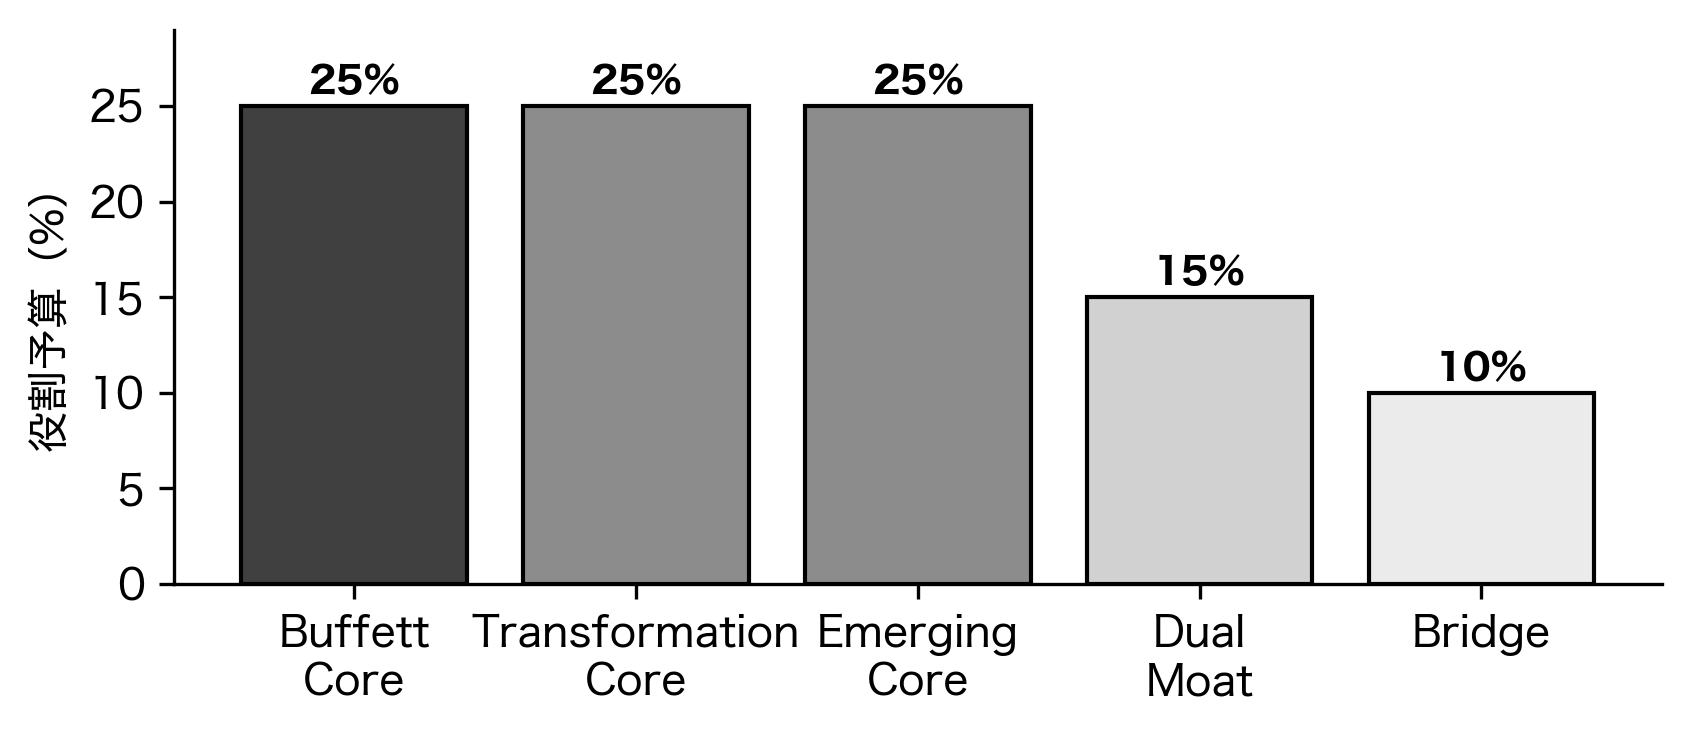
\includegraphics[width=0.8\linewidth]{p4_role_budget.png}
\caption{役割予算。三世代に各 25\%，両立型 15\%，分散役 10\%。}
\label{fig:budget}
\end{figure}

% ---------- 4 ----------
\section{役割内の傾け：リスク調整配分}
\label{sec:tilt}

\begin{keybox}[フローでの位置]
式\eqref{eq:alloc}は，役割予算を各銘柄へ配る唯一の式である。銘柄の入れ替えには一切関与しない。使う情報は，値動きの大きさ・売買のしやすさ・証拠の強さ・データの信頼度の四つで，いずれも「将来のリターン」ではない。
\end{keybox}

\begin{equation}
\omega_i \;=\; B_{r(i)}\cdot\frac{\rho_i}{\displaystyle\sum_{j:\,r(j)=r(i)}\rho_j},
\qquad
\rho_i \;=\; \frac{\ell_i\, e_i\, c_i}{\max(\sigma_i,\,0.10)}.
\label{eq:alloc}
\end{equation}

ここで $r(i)$ は銘柄 $i$ の役割，$B_r$ は役割予算である。傾け係数 $\rho_i$ の部品は表\ref{tab:coef}の通りで，すべて実装値である。

\begin{table}[H]
\caption{傾け係数の部品（実装値）}
\label{tab:coef}
\centering
\small
\begin{tabularx}{\linewidth}{p{18mm}p{40mm}Y}
\toprule
記号 & 名称 & 実装 \\
\midrule
$\sigma_i$ & 値動きの大きさ & 直近 1 年の日次収益率の年率標準偏差。下限 0.10 でクリップ（小さすぎる $\sigma$ で配分が暴れるのを防ぐ）。 \\
$\ell_i$ & 流動性係数 & 60 日平均売買代金が 5{,}000 万円以上で 1.00，3{,}000 万円以上で 0.85，未満で 0.70。 \\
$e_i$ & 証拠係数 & $1+0.05\times(\text{Evidence Level}-2)$。L3 は 1.05，L2 は 1.00，L1 は 0.95。 \\
$c_i$ & 信頼度係数 & $0.5+0.5\times\text{Phase2 信頼度}$。データの確からしさで 0.5〜1.05。 \\
\bottomrule
\end{tabularx}
\end{table}

\begin{defbox}
$\rho_i$ は「安心して多めに置ける度合い」である。分母の $\sigma_i$ が大きい（値動きが荒い）ほど配分は減り，分子の三係数が高い（流動・証拠・信頼）ほど配分は増える。リターン予想が入っていないことに注意してほしい。
\end{defbox}

% ---------- 5 ----------
\section{8\%上限と配り直しの手順}
\label{sec:cap}

一銘柄への集中を防ぐため，$\omega_i$ には 8\% の上限を課す。上限を超えた場合の配り直しは，次の決定的な手順で行う（実装と一致）。

\begin{enumerate}
\item $\omega_i>8\%$ の銘柄を 8\% へ切り下げる。
\item 切り下げで生じた余剰を，同じ役割内の未上限銘柄へ，現行比率に比例して配り直す。
\item 配り直しで新たに 8\% を超える銘柄が出れば，手順 1--2 を繰り返す（最大 5 回）。
\item 役割間の移動や現金化は行わない（役割予算を保存する）。
\end{enumerate}

なお本ポートフォリオでは，役割内が最少でも 2 銘柄・役割予算最大 25\% のため，全銘柄が上限に張り付いて配りきれない状況は構成上生じない。

% ---------- 6 ----------
\section{単元株調整：実際に買える株数へ丸める}
\label{sec:lot}

目標比率 $\omega_i$ は連続量だが，株は最小売買単位（単元）でしか買えない。実購入株数は次で決める。

\begin{equation}
q_i \;=\; L_i\cdot\operatorname{floor}\!\left(\frac{B\,\omega_i}{P_i\,L_i}\right).
\label{eq:lot}
\end{equation}

$q_i$ は購入株数，$L_i$ は売買単位，$B=500$ 万円は総予算，$P_i$ は株価，$\operatorname{floor}$ は切り捨てである。切り捨てで生じた端数は残現金として保持する（他銘柄へ再配分しない）。

基準ケースは $L_i=1$（単元未満株＝S 株の利用を仮定）であり，20 社すべてが購入可能で消化率は 99.0\% となる。感度ケース $L_i=100$（実単元）では，株価の高い 9 社が「1 単元の金額が予算 8\% を超える」等の理由で購入できず，消化率は 46.7\% まで低下する。実運用では単元未満株の利用が前提であり，その可否は課題規約で確認を要する（人間確認事項）。

\begin{figure}[H]
\centering
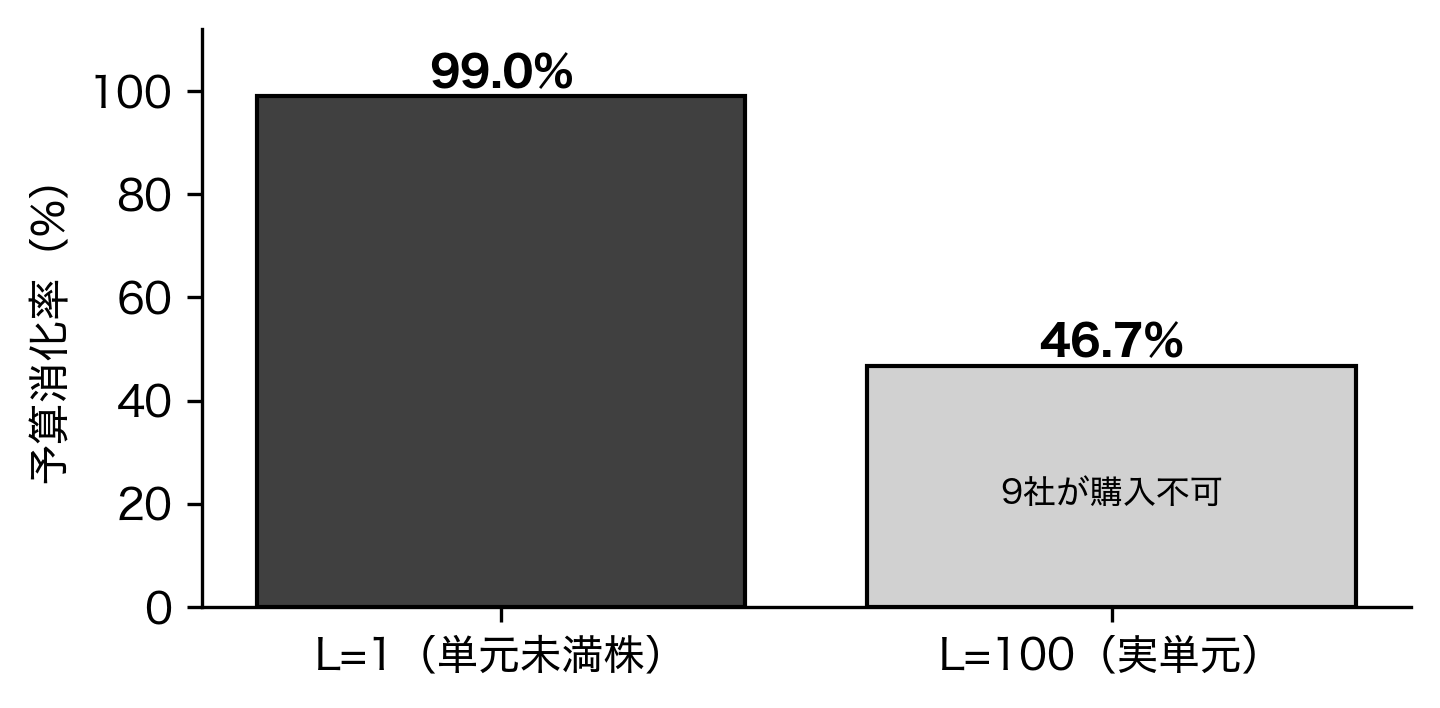
\includegraphics[width=0.62\linewidth]{p4_lot.png}
\caption{単元の仮定と予算消化率。L=1 で 99.0\%，L=100 では 9 社が購入不可となり 46.7\%。}
\label{fig:lot}
\end{figure}

% ---------- 7 ----------
\section{執行結果と制約の確認}

最終配分（C 案）の執行結果は次の通りである。投資額 4{,}949{,}198 円・残現金 50{,}801 円（消化率 99.0\%）。最大保有は 9474 ゼンリンの 7.46\%（上限 8\% 内），業種の最大は 17.3\%（上限 25\% 内），テーマの最大は 16.2\%（上限 25\% 内）。目標比率との最大乖離は 0.3 ポイントに収まった。

\subsection{ミニ演習：上限にかかったらどうなるか}

仮に，ある役割（予算 25\%・5 社）で $\rho$ 比が突出した 1 社の $\omega$ が 9\% と計算されたとする。手順により当該社は 8\% へ切り下げられ，余剰 1\% は同役割の残り 4 社へ現行比率で配り直される。役割合計は 25\% のまま保たれる。役割の外へは漏れない——これが「役割予算の保存」である。

% ---------- 8 ----------
\section{計算例：一社を0から配分する}
\label{sec:example}

9470 学研ホールディングス（完成した堀）を実測値で追う。値動き $\sigma$ は約 0.20 と穏やかで，60 日売買代金は約 1.2 億円（$\ell=1.00$），Evidence Level は L3（$e=1.05$），Phase2 信頼度は 0.98（$c\approx0.99$）。よって $\rho$ は役割内で高めとなり，目標比率は $\omega=6.88\%$ と計算された。金額では $500\text{万円}\times6.88\%=343{,}946$ 円。株価 941 円で式\eqref{eq:lot}を適用すると $q=\operatorname{floor}(343{,}946/941)=365$ 株，実購入額は $941\times365=343{,}465$ 円。端数 481 円は残現金に积まれる。

% ---------- 9 ----------
\section{限界と誠実な書き方}
\label{sec:limits}

\begin{itemize}
\item $\sigma_i$ は過去 1 年の値であり，将来の値動きを保証しない。
\item 係数（$0.05$，$0.5$ など）は設計値であり，最適化した係数ではない。
\item $L=1$ は単元未満株の利用を仮定する。認められない場合は $L=100$ 前提の代替配分が必要で，9 社が購入不可となる。
\item 配分は分散と執行可能性を整えるだけで，リターンを高める仕組みではない。
\end{itemize}

\subsection{本文で使える要約文}
\begin{keybox}
配分は，選定済み 20 社に対して役割予算（完成・変化・新生 各 25\%，両立型 15\%，分散役 10\%）を置き，役割内では値動き・流動性・証拠水準・データ信頼度のみで傾けた（リターン予想は不使用）。1 銘柄 8\% 上限の超過分は同一役割内で配り直し，単元株の切り捨て端数は残現金とした。単元未満株（L=1）で投資額 4{,}949{,}198 円・消化率 99.0\%，実単元（L=100）では 9 社が購入不可となるため，単元未満株の利用を前提とする。
\end{keybox}

% ---------- Appendix ----------
\newpage
\section{Appendix A：変数一覧}
\begin{longtable}{p{24mm}p{44mm}p{76mm}}
\caption{Phase4 で使う主な変数}\\
\toprule
記号 & 名称 & 意味 \\
\midrule
\endfirsthead
\toprule
記号 & 名称 & 意味 \\
\midrule
\endhead
$\omega_i$ & 目標比率 & ポートフォリオに占める銘柄 $i$ の割合（上限 8\%）。 \\
$B_r$ & 役割予算 & 役割 $r$ への配分枠。25/25/25/15/10\%。 \\
$\rho_i$ & 傾け係数 & 役割内の配分優先度。$\ell e c/\max(\sigma,0.10)$。 \\
$\sigma_i$ & 年率ボラティリティ & 直近 1 年日次収益率の標準偏差（下限 0.10）。 \\
$\ell_i$ & 流動性係数 & 売買代金 5{,}000 万↑=1.00／3{,}000 万↑=0.85／未満=0.70。 \\
$e_i$ & 証拠係数 & $1+0.05(\text{Level}-2)$。 \\
$c_i$ & 信頼度係数 & $0.5+0.5\times$Phase2 信頼度。 \\
$q_i$ & 購入株数 & 式\eqref{eq:lot}。切り捨てで単元へ丸める。 \\
$L_i$ & 売買単位 & 基準 1 株（単元未満株）／感度 100 株。 \\
$B$ & 総予算 & 500 万円。 \\
$P_i$ & 株価 & 2026-06-01 終値。 \\
\bottomrule
\end{longtable}

\section{References}
\begin{itemize}
\item Markowitz, H. (1952). Portfolio Selection. \emph{Journal of Finance}, 7(1), 77--91.
\item 日本取引所グループ「単元株制度」（売買単位に関する制度解説）．
\end{itemize}

\end{document}
